\subsection{FPGA Acceleration}\label{section: fpga-acceleration}

The NTT acceleration design consists of two main parts: the NTT engine and the DMA data transfer engine. The NTT engine performs calculations on given-length data points, while the DMA data transfer engine efficiently exchanges data between the NTT engine and DDR.

\begin{figure}[ht]
  \centering
  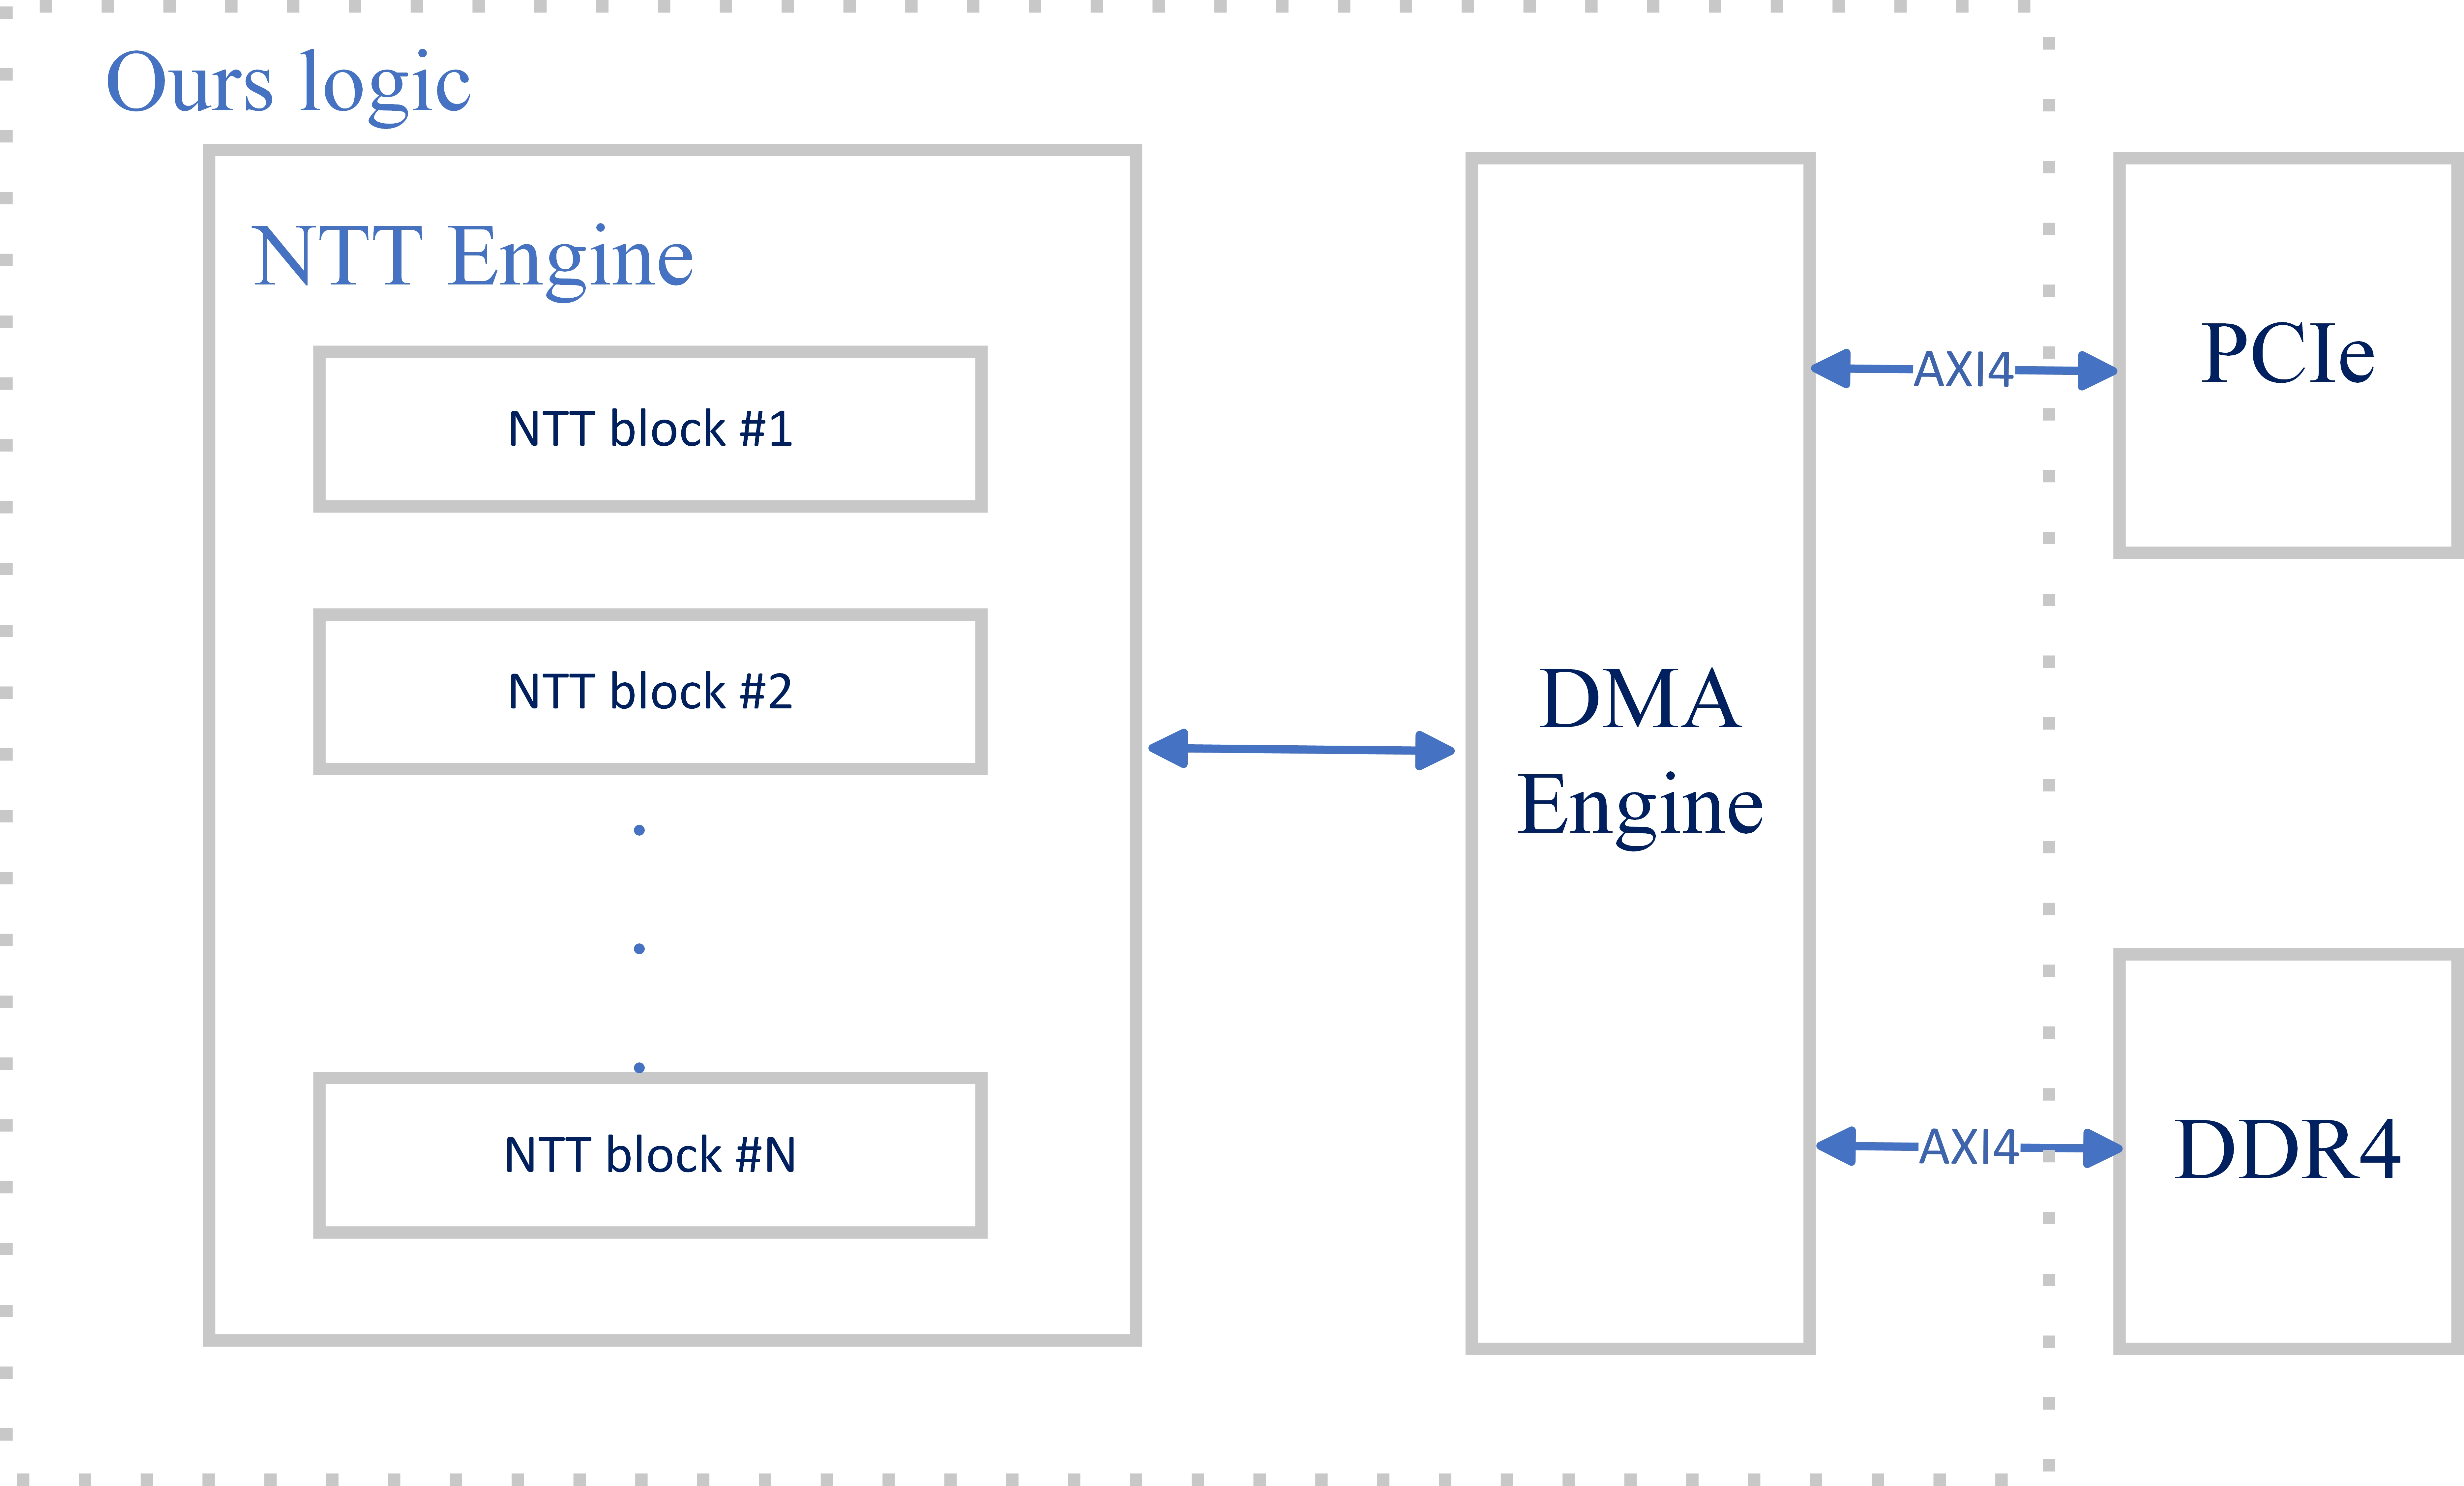
\includegraphics[width=0.8\textwidth]{The design of NTT acceleration implemented in FPGA.jpg}
  \caption{The design of NTT acceleration implemented in FPGA}
  \label{fig:The design of NTT acceleration implemented in FPGA}
\end{figure}

\subsubsection{NTT engine}

In this design, the NTT engine consists of multiple parallel-running NTT modules. The maximum supported data length for a single NTT module is $2^{12}$. Moreover, a  modular multiplication unit is connected to the output of each NTT module to support the extension of two-dimensional or higher-dimensional NTTs. To improve scalability performance, variable-length NTT calculations can be achieved through parameter configuration through the AXI4 interface.

In practical applications, processing in parallel with multiple NTT modules can greatly improve computational performance. For a single NTT module, one point reading and one storage operation are required per clock cycle. When 8 NTTs are processed in parallel in the engine, the total access bandwidth required is 8 * 8 byte/point * (1x read + 1x write) * 100MHz = 11.92 GB/sec with assuming a working clock of 100MHz. That is, the calculation rate of NTT is 8 * 100MHz / $2^{24}$ / 2= 25 times/sec. For the AWS FPGA platform, the user logic can use three DDR4 channels with a interface frequency up to 2100MHz. The total supported simultaneous access bandwidth is 3 * 8 byte/DDR * 2100MHz = 46.9 GB/sec. Therefore, the maximum supported NTT calculation rate is 25 * 46.9 / 11.92 = 98 times/sec.


\subsubsubsection{NTT calculation module}

To support NTT calculation with the length of $2^{24}$, it is better to consider the $2^{24}$ points as a 2D array with a size of $2^{12}$ points by $2^{12}$ points. Using the Gentleman-Sande algorithm, the first pass through the engine computes $2^{12}$ NTTs column-wise of the 2D array using the carefully designed NTT module with a length of $2^{12}$. For this module, a recursive NTT Algorithm is adopted, which contains 12 stages of butterfly with varying kernel sizes. Users can adjust the sizes of both columns and rows in the 2D array by setting parameters to meet FPGA running requirements. Finally, the output of the NTT block performs modular multiplication according to the 2D NTT algorithm.

\begin{figure}[ht]
  \centering
  
\includegraphics[width=1\textwidth]{Various-size NTT block.jpg}
  \caption{Various-size NTT block (MM: modular multiplication)}
  \label{fig:NTT_module}
\end{figure}

\subsubsubsection{NTT kernel}
The NTT block contains several kernels, each of which is mainly composed of a butterfly unit and two RAMs. The butterfly unit is carefully designed to take maximum advantage of the FPGA DSPs, especially by utilizing the tricks of the Goldilocks field multiply to improve computational efficiency over modular reduction. One of the RAMs is used to buffer the input data, while the other stores the twiddle factors required for butterfly calculation.


\begin{figure}[ht]
  \centering
  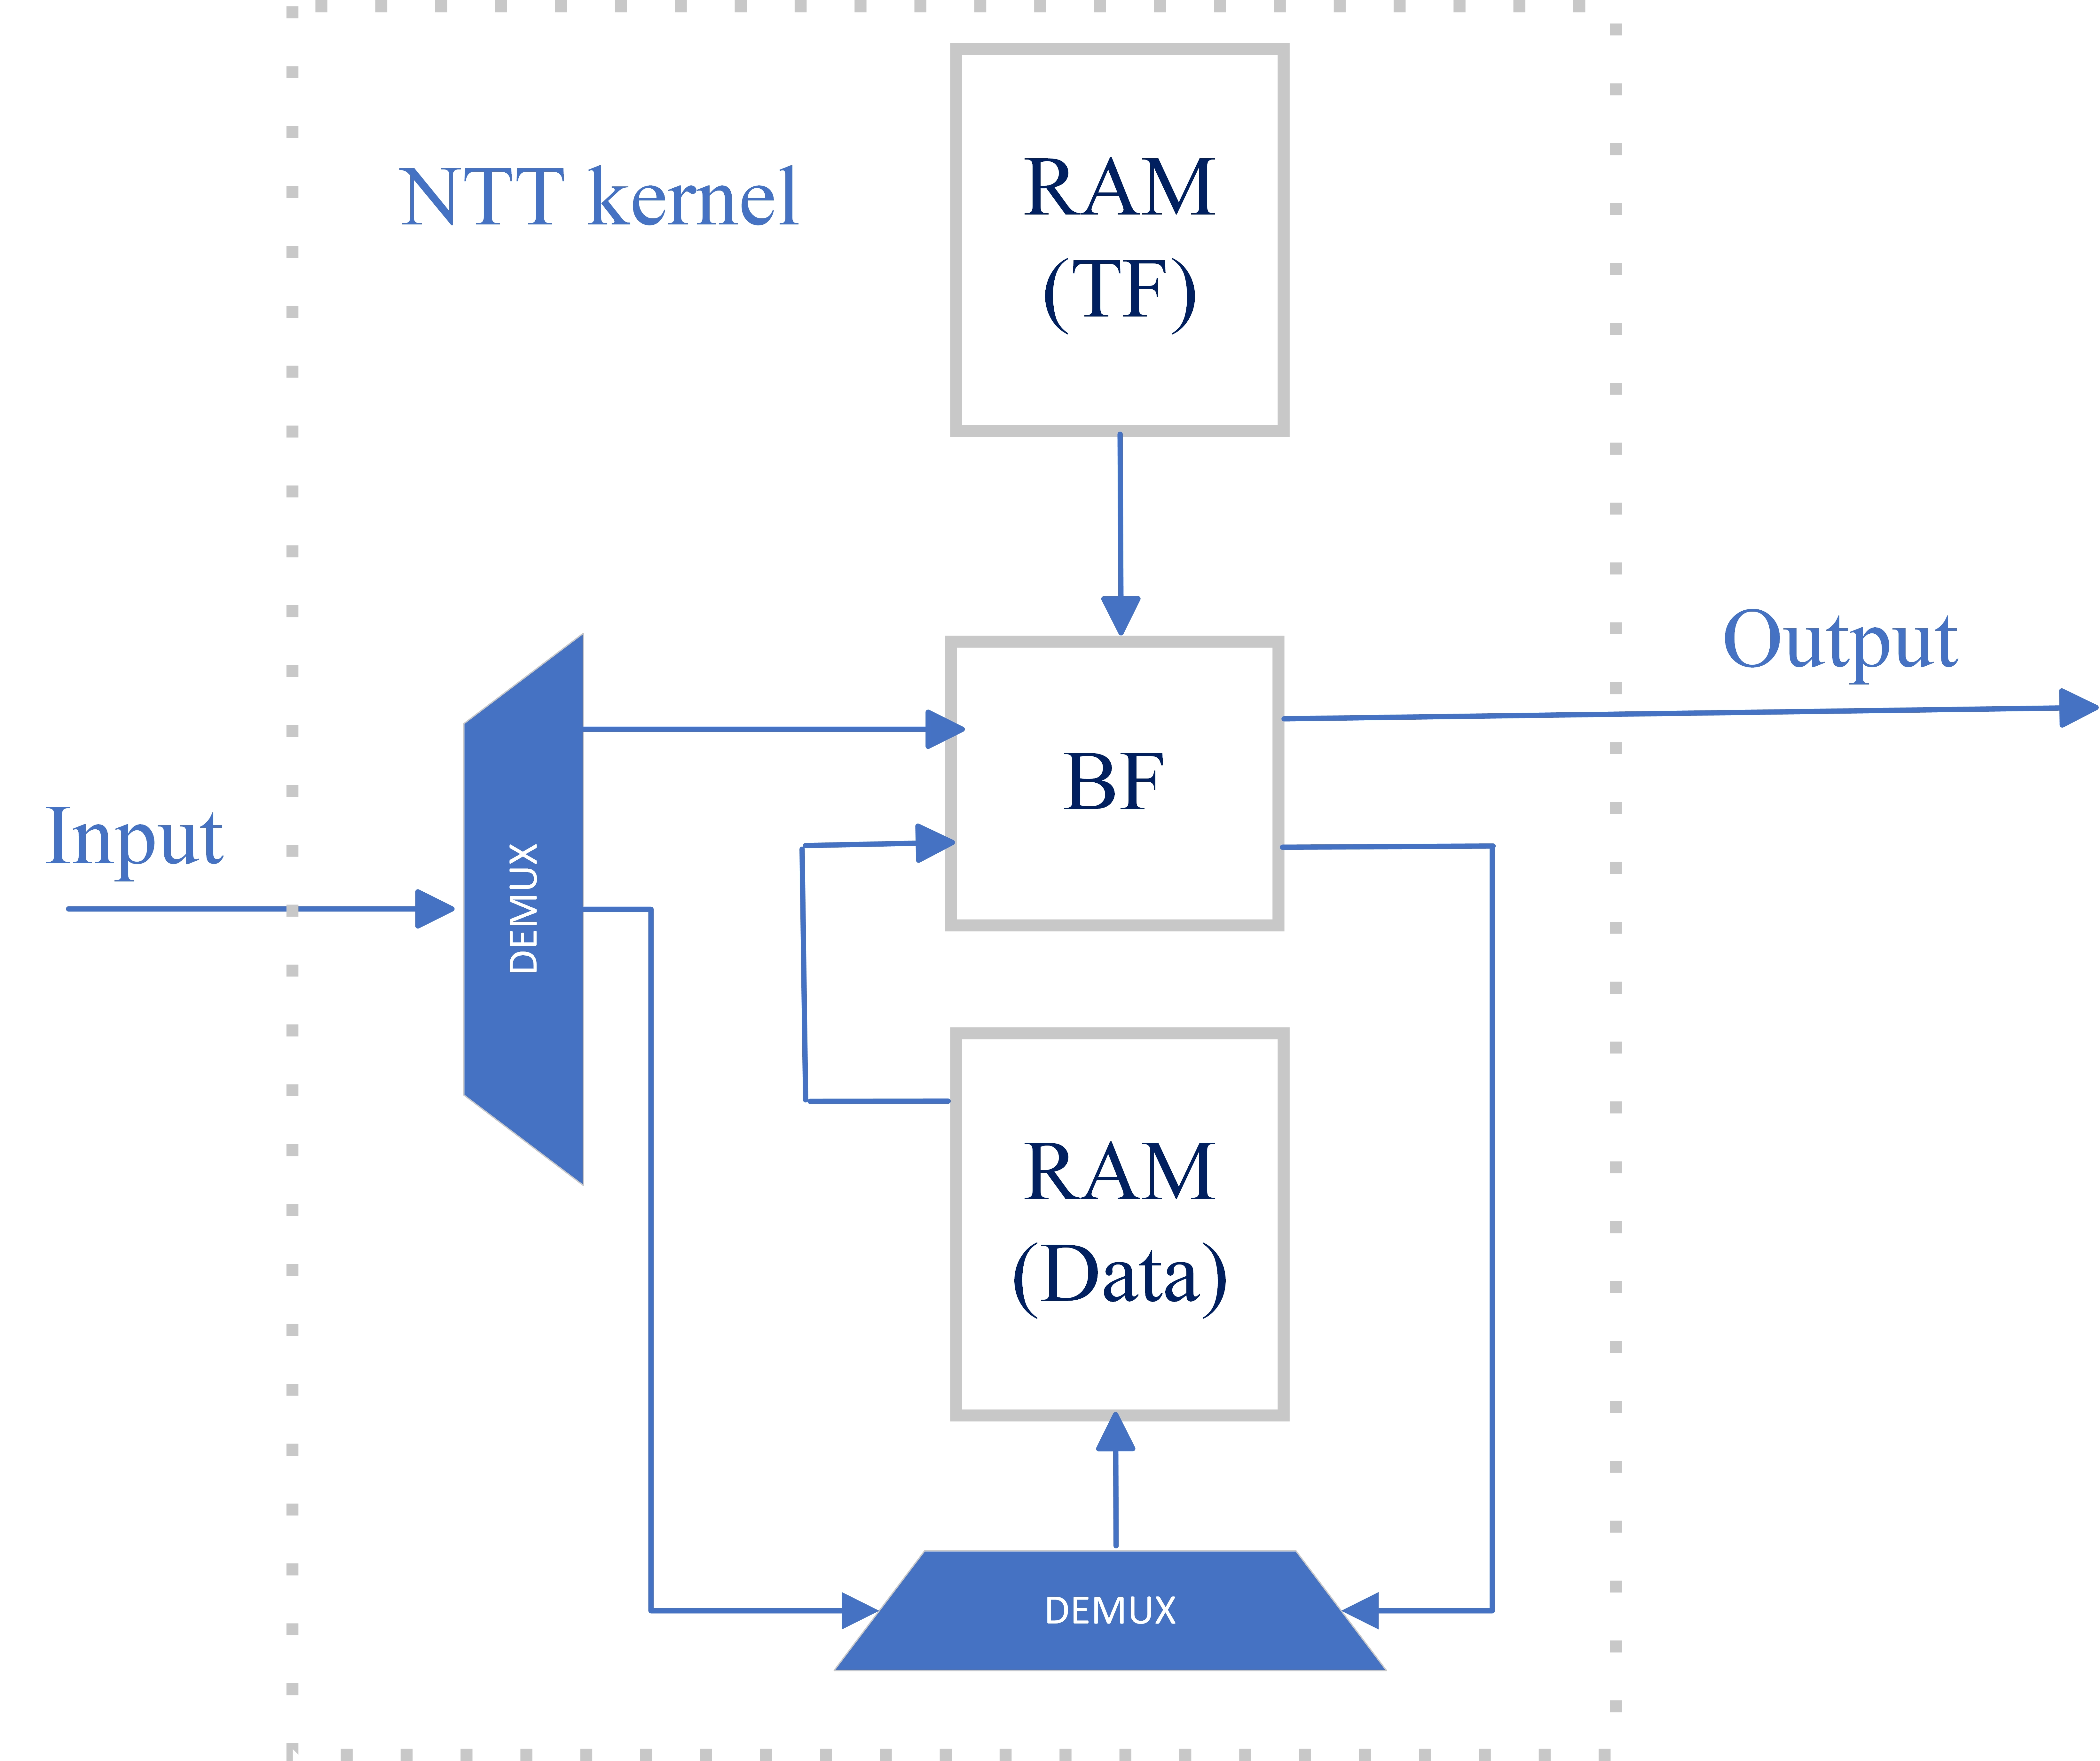
\includegraphics[width=0.5\textwidth]{NTT kernel.jpg}
  \caption{NTT kernel (TF: twiddle factor; BF: Butterfly)}
  \label{fig:NTT_kernel}
\end{figure}

\subsubsubsection{Generation of twiddle factors}

To realize the 2D NTT, the outputs of the 1st pass with the NTT engine should be multiplied by the corresponding twiddle factors, as shown in Fig.2. Since the twiddle factors required for the NTT output of different columns of the 2D array are different, these twiddle factors must be updated for every column. To reduce the necessary DDR bandwidth, a combination of LUT and computation is used to generate these twiddle factors. The LUT provides  $2^{12}$ twiddles needed for modular multiplication before the 2nd pass.Then, the updating twiddle factor is computed by multiplying the LUT twiddles with an accumulated running twiddle factor and then writing back to the LUTs at the same of modular multiplying. Additionally, the twiddle factors needed in the NTT block are provided by LUTs and loaded once before performing the NTT. Therefore, the total number of multiplication/reduction units per block is 13: 11 for the 12 butterfly stages and 2 for each twiddle updating and modulation multiplication out of the NTT block.

\subsubsubsection{Bit Reversal}
The NTT engine performs bit reversal during NTT computation, which is achieved by bit reversing each pass of the NTT at the end of the block (as shown in the above NTT blocks). A final step is required to complete the bit reversal across the two passes. This can be achieved by writing back the results of the 2nd pass using the column-major access pattern instead of the row-major access pattern.


\subsubsection{DMA Engine}

The sole responsibility of the DMA Engine is to exchange points between the NTT Engine and the memory outside of the FPGA at the NTT Engine's burst processing rate. With the NTT Engine capable of consuming and producing 8 points per cycle when 8 NTT blocks are working concurrently, and an NTT Engine clock rate nearing 300MHz, the feed and sink rates are both 17.9 GB/sec. The FPGA's DDR4 memory, with a peak bandwidth of 46.9 GB/sec, can support the combined feed and sink bandwidth need of 35.8 GB/sec while also providing enough storage for $2^{24}$ points.
  In addition, to fully utilize the bandwidth of DDR4 and continuously provide high data bandwidth to the NTT engine, a large data buffer RAM is introduced in the DMA engine to maintain a high data throughput rate for the AXI4 interface.

\subsubsection{Simulation}

To verify the feasibility of the designed NTT acceleration scheme, it was implemented in Vivado using Verilog HDL language and both functional and timing simulations were performed. The simulation results are shown in the following figure.

\begin{figure}[h]
  \centering
  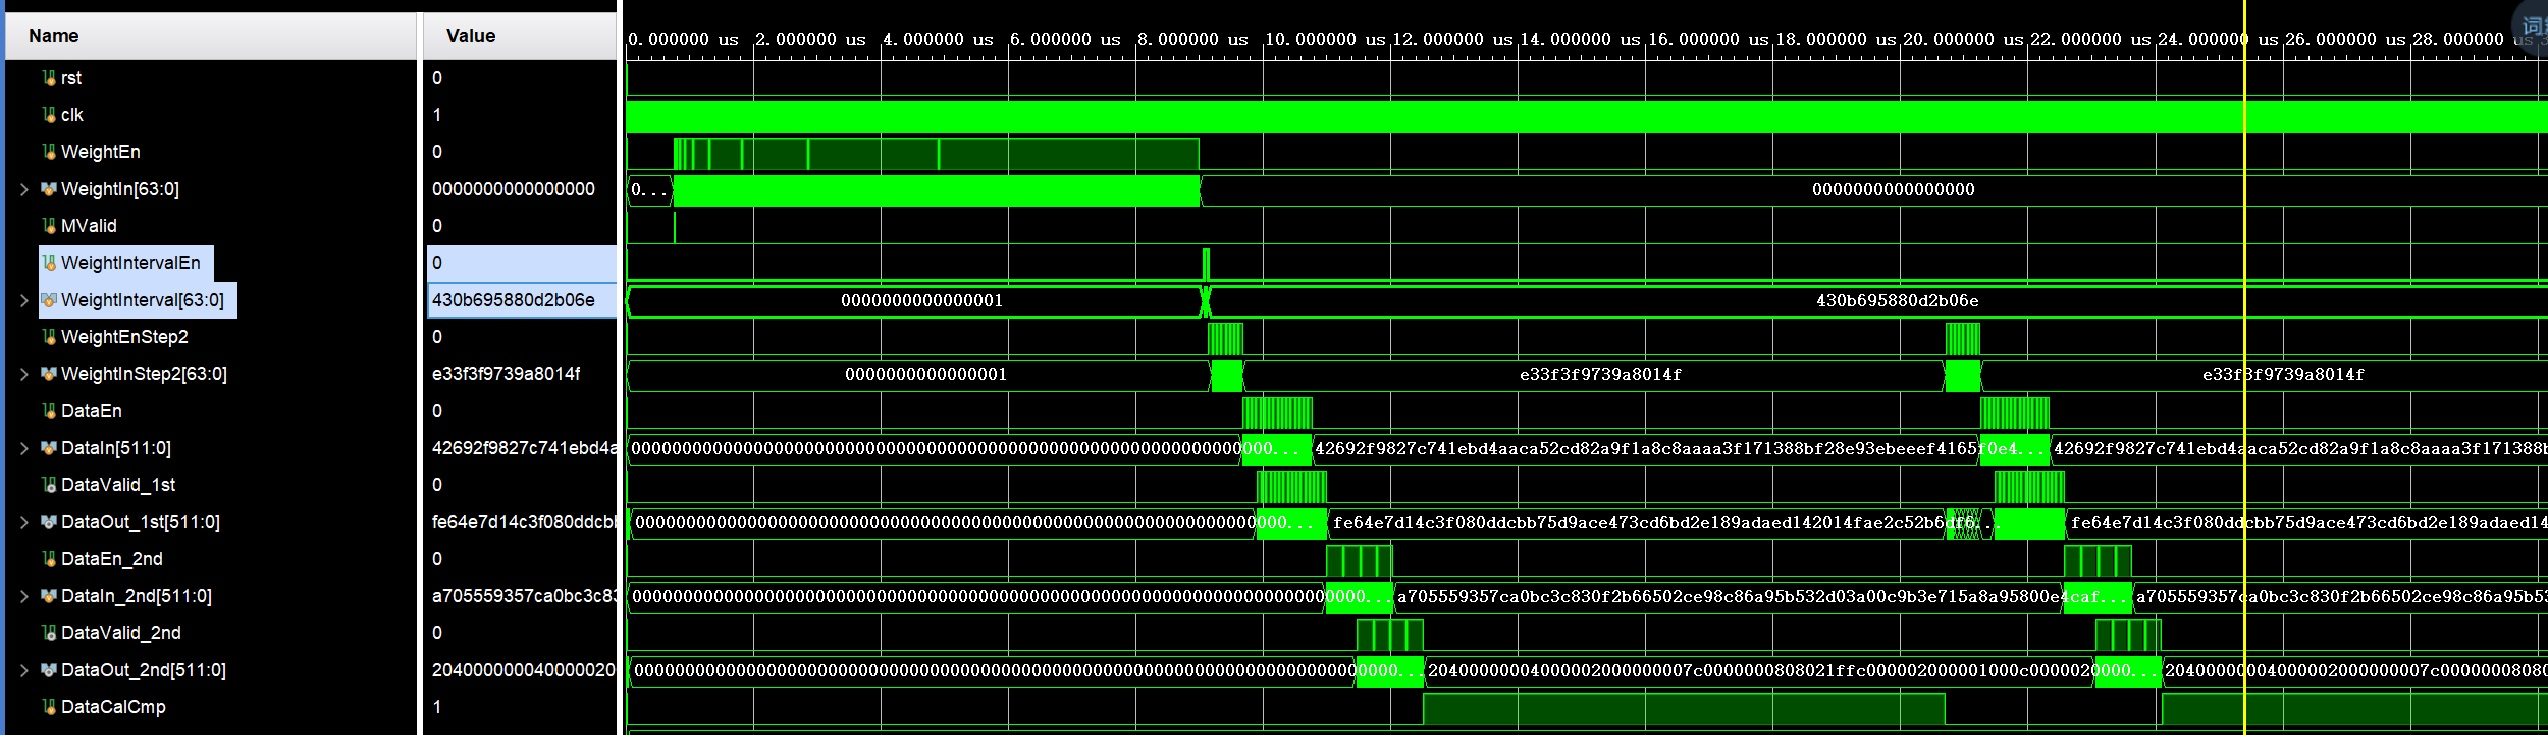
\includegraphics[width=1\textwidth]{NTT simulation.jpg}
  \caption{NTT simulation}
  \label{fig:NTT_Simu}
\end{figure}

In the Figure: the signals of WeightEn and WeightIn are the configurations for the twiddle factors of the NTT module; WeightEnStep2 and WeightInStep2 are twiddle factors for the output of large number modular multiplication in the NTT module; signals of WeightIntervalEn and WeightIntervalIn are used to be accumulated twiddle factors when updating the twiddle to multiply the outputs of NTT blocks; DataIn and DataEn are the input data for the first dimension of the NTT, while DataOut\_1st and DataValid\_1st are the computed results outputted; DataIn\_2nd and DataEn\_2nd are the input data for the second dimension of the NTT, and DataOut\_2nd and DataValid\_2nd are the computed results outputted; DataCalCmp is used for indicate the comparison of the computed NTT results with the theoretical ones.

In the implementation, 8-way parallel NTT acceleration is used. According to the timing, the NTT engine is respectively configured with LUT twiddle factors, LUT twiddle factors of modular multiplication, and accumulated twiddle factors. To compute a 4096-point NTT, the size of the 2D array is 8 * 16 * 32 for the first passs and 8 * 4 * 128 for the second one. Based on the comparison signal DataCalCmp, the results obtained from the 2D NTT operation are consistent with the theoretical values. When performing the second 4096-point NTT acceleration, it is only necessary to reload the modular multiplication LUT twiddle factors.
